% Portfolio Optimization: Modern Portfolio Theory
% Topics: Mean-variance optimization, efficient frontier, CAPM, Sharpe ratio, risk measures
% Style: Quantitative finance research report with computational analysis

\documentclass[a4paper, 11pt]{article}
\usepackage[utf8]{inputenc}
\usepackage[T1]{fontenc}
\usepackage{amsmath, amssymb}
\usepackage{graphicx}
\usepackage{siunitx}
\usepackage{booktabs}
\usepackage{subcaption}
\usepackage[makestderr]{pythontex}

% Theorem environments
\newtheorem{definition}{Definition}[section]
\newtheorem{theorem}{Theorem}[section]
\newtheorem{example}{Example}[section]
\newtheorem{remark}{Remark}[section]

% Load hyperref LAST with hidelinks option
\usepackage[hidelinks]{hyperref}

\title{Portfolio Optimization: Modern Portfolio Theory and Risk Management}
\author{Quantitative Finance Research Group}
\date{\today}

\begin{document}
\maketitle

\begin{abstract}
This report presents a comprehensive computational analysis of portfolio optimization using
Modern Portfolio Theory (MPT). We examine the mean-variance framework introduced by Markowitz,
construct efficient frontiers for multi-asset portfolios, derive optimal portfolio weights under
various constraints, and analyze risk-adjusted performance using the Sharpe ratio. The analysis
includes Value-at-Risk (VaR) and Conditional Value-at-Risk (CVaR) computations, demonstrating
the practical implementation of quadratic programming for portfolio construction with realistic
constraints including long-only positions and sector allocation limits.
\end{abstract}

\section{Introduction}

Modern Portfolio Theory, pioneered by Harry Markowitz in 1952, revolutionized investment
management by formalizing the trade-off between expected return and risk. The fundamental
insight is that portfolio risk depends not only on individual asset volatilities but also
on the correlation structure between assets. By carefully selecting portfolio weights,
investors can achieve superior risk-adjusted returns compared to naive diversification strategies.

\begin{definition}[Portfolio Return and Risk]
For a portfolio with $n$ assets, let $\mathbf{w} = (w_1, \ldots, w_n)^T$ denote the vector
of portfolio weights, where $\sum_{i=1}^n w_i = 1$. The expected portfolio return is:
\begin{equation}
\mu_p = \mathbf{w}^T \boldsymbol{\mu}
\end{equation}
where $\boldsymbol{\mu} = (\mu_1, \ldots, \mu_n)^T$ is the vector of expected asset returns.
The portfolio variance is:
\begin{equation}
\sigma_p^2 = \mathbf{w}^T \boldsymbol{\Sigma} \mathbf{w}
\end{equation}
where $\boldsymbol{\Sigma}$ is the $n \times n$ covariance matrix of asset returns.
\end{definition}

\section{Theoretical Framework}

\subsection{Mean-Variance Optimization}

The Markowitz mean-variance optimization problem seeks to minimize portfolio risk for a
given level of expected return, or equivalently, maximize expected return for a given risk level.

\begin{theorem}[Markowitz Optimization Problem]
The minimum variance portfolio for a target return $\mu_{\text{target}}$ solves:
\begin{equation}
\begin{aligned}
\min_{\mathbf{w}} \quad & \frac{1}{2}\mathbf{w}^T \boldsymbol{\Sigma} \mathbf{w} \\
\text{s.t.} \quad & \mathbf{w}^T \boldsymbol{\mu} = \mu_{\text{target}} \\
& \mathbf{w}^T \mathbf{1} = 1
\end{aligned}
\end{equation}
where $\mathbf{1}$ is a vector of ones. Additional constraints may include $w_i \geq 0$
(long-only) or sector allocation limits.
\end{theorem}

\subsection{The Efficient Frontier}

\begin{definition}[Efficient Frontier]
The efficient frontier is the set of portfolios that offer the maximum expected return for
each level of risk (variance). Portfolios on the efficient frontier dominate all other
portfolios with the same risk but lower return, or same return but higher risk.
\end{definition}

\begin{theorem}[Two-Fund Separation]
Any portfolio on the efficient frontier can be expressed as a linear combination of two
frontier portfolios. In particular, with a risk-free asset, any efficient portfolio is a
combination of the risk-free asset and the tangency portfolio (market portfolio).
\end{theorem}

\subsection{Capital Asset Pricing Model}

\begin{definition}[CAPM]
The Capital Asset Pricing Model relates expected return to systematic risk:
\begin{equation}
E[R_i] = R_f + \beta_i (E[R_m] - R_f)
\end{equation}
where $R_f$ is the risk-free rate, $R_m$ is the market return, and $\beta_i$ is the asset's
systematic risk coefficient:
\begin{equation}
\beta_i = \frac{\text{Cov}(R_i, R_m)}{\text{Var}(R_m)}
\end{equation}
\end{definition}

\subsection{Risk-Adjusted Performance}

\begin{definition}[Sharpe Ratio]
The Sharpe ratio measures risk-adjusted return:
\begin{equation}
\text{Sharpe Ratio} = \frac{\mu_p - R_f}{\sigma_p}
\end{equation}
Higher Sharpe ratios indicate superior risk-adjusted performance. The tangency portfolio
maximizes the Sharpe ratio among all risky portfolios.
\end{definition}

\subsection{Risk Measures}

\begin{definition}[Value-at-Risk]
The Value-at-Risk (VaR) at confidence level $\alpha$ is the maximum loss not exceeded with
probability $\alpha$:
\begin{equation}
\text{VaR}_\alpha = -\inf\{x : P(L \leq x) \geq \alpha\}
\end{equation}
For normally distributed returns, $\text{VaR}_\alpha = -(\mu_p - z_\alpha \sigma_p)$ where
$z_\alpha$ is the $\alpha$-quantile of the standard normal distribution.
\end{definition}

\begin{definition}[Conditional Value-at-Risk]
The Conditional Value-at-Risk (CVaR), also called Expected Shortfall, is the expected loss
given that the loss exceeds VaR:
\begin{equation}
\text{CVaR}_\alpha = E[L \mid L \geq \text{VaR}_\alpha]
\end{equation}
CVaR is a coherent risk measure and provides information about tail risk beyond VaR.
\end{definition}

\section{Computational Implementation}

We now implement portfolio optimization for a realistic multi-asset portfolio. We consider
six assets representing different asset classes: large-cap equity, small-cap equity,
international equity, corporate bonds, government bonds, and real estate investment trusts (REITs).
Historical return data inform our estimates of expected returns and the covariance matrix.

\begin{pycode}
import numpy as np
import matplotlib.pyplot as plt
from scipy.optimize import minimize, LinearConstraint, Bounds
from scipy.stats import norm
import warnings
warnings.filterwarnings('ignore')

np.random.seed(42)

# Asset names
asset_names = ['Large Cap', 'Small Cap', 'International', 'Corp Bonds', 'Gov Bonds', 'REITs']
n_assets = len(asset_names)

# Expected annual returns (%) - based on historical data
expected_returns = np.array([10.5, 12.0, 11.2, 5.5, 3.2, 8.5])

# Annual volatilities (%)
volatilities = np.array([18.0, 25.0, 22.0, 8.0, 5.0, 20.0])

# Correlation matrix (realistic values)
correlation_matrix = np.array([
    [1.00, 0.85, 0.75, 0.25, 0.10, 0.55],
    [0.85, 1.00, 0.70, 0.20, 0.05, 0.60],
    [0.75, 0.70, 1.00, 0.30, 0.15, 0.50],
    [0.25, 0.20, 0.30, 1.00, 0.80, 0.35],
    [0.10, 0.05, 0.15, 0.80, 1.00, 0.20],
    [0.55, 0.60, 0.50, 0.35, 0.20, 1.00]
])

# Construct covariance matrix
cov_matrix = np.outer(volatilities, volatilities) * correlation_matrix

# Risk-free rate
risk_free_rate = 2.5

# Function to calculate portfolio statistics
def portfolio_stats(weights, returns, cov_matrix, rf_rate):
    """Calculate portfolio return, volatility, and Sharpe ratio."""
    port_return = np.dot(weights, returns)
    port_volatility = np.sqrt(np.dot(weights, np.dot(cov_matrix, weights)))
    sharpe_ratio = (port_return - rf_rate) / port_volatility
    return port_return, port_volatility, sharpe_ratio

# Minimum variance portfolio (unconstrained)
def min_variance_portfolio(cov_matrix):
    """Find the global minimum variance portfolio."""
    n = len(cov_matrix)
    # Objective: minimize variance
    def objective(w):
        return np.dot(w, np.dot(cov_matrix, w))

    # Constraint: weights sum to 1
    constraints = {'type': 'eq', 'fun': lambda w: np.sum(w) - 1}

    # Initial guess: equal weights
    w0 = np.ones(n) / n

    result = minimize(objective, w0, method='SLSQP', constraints=constraints)
    return result.x

# Minimum variance portfolio (long-only)
def min_variance_portfolio_long_only(cov_matrix):
    """Find the minimum variance portfolio with long-only constraint."""
    n = len(cov_matrix)
    def objective(w):
        return np.dot(w, np.dot(cov_matrix, w))

    constraints = {'type': 'eq', 'fun': lambda w: np.sum(w) - 1}
    bounds = Bounds(0, 1)  # Long-only constraint
    w0 = np.ones(n) / n

    result = minimize(objective, w0, method='SLSQP', constraints=constraints, bounds=bounds)
    return result.x

# Tangency portfolio (maximum Sharpe ratio)
def tangency_portfolio(returns, cov_matrix, rf_rate):
    """Find the tangency portfolio (maximum Sharpe ratio)."""
    n = len(returns)

    def neg_sharpe(w):
        ret, vol, sharpe = portfolio_stats(w, returns, cov_matrix, rf_rate)
        return -sharpe  # Minimize negative Sharpe = maximize Sharpe

    constraints = {'type': 'eq', 'fun': lambda w: np.sum(w) - 1}
    bounds = Bounds(0, 1)
    w0 = np.ones(n) / n

    result = minimize(neg_sharpe, w0, method='SLSQP', constraints=constraints, bounds=bounds)
    return result.x

# Efficient frontier portfolio for target return
def efficient_portfolio(returns, cov_matrix, target_return):
    """Find minimum variance portfolio for a target return (long-only)."""
    n = len(returns)

    def objective(w):
        return np.dot(w, np.dot(cov_matrix, w))

    constraints = [
        {'type': 'eq', 'fun': lambda w: np.sum(w) - 1},
        {'type': 'eq', 'fun': lambda w: np.dot(w, returns) - target_return}
    ]
    bounds = Bounds(0, 1)
    w0 = np.ones(n) / n

    result = minimize(objective, w0, method='SLSQP', constraints=constraints, bounds=bounds)
    if result.success:
        return result.x
    else:
        return None

# Calculate key portfolios
weights_min_var = min_variance_portfolio_long_only(cov_matrix)
weights_tangency = tangency_portfolio(expected_returns, cov_matrix, risk_free_rate)

# Equal weight portfolio for comparison
weights_equal = np.ones(n_assets) / n_assets

# Calculate statistics for key portfolios
ret_min_var, vol_min_var, sharpe_min_var = portfolio_stats(
    weights_min_var, expected_returns, cov_matrix, risk_free_rate)
ret_tangency, vol_tangency, sharpe_tangency = portfolio_stats(
    weights_tangency, expected_returns, cov_matrix, risk_free_rate)
ret_equal, vol_equal, sharpe_equal = portfolio_stats(
    weights_equal, expected_returns, cov_matrix, risk_free_rate)

# Generate efficient frontier
target_returns = np.linspace(ret_min_var, expected_returns.max() * 0.95, 50)
efficient_portfolios = []
efficient_vols = []

for target in target_returns:
    weights = efficient_portfolio(expected_returns, cov_matrix, target)
    if weights is not None:
        efficient_portfolios.append(weights)
        _, vol, _ = portfolio_stats(weights, expected_returns, cov_matrix, risk_free_rate)
        efficient_vols.append(vol)

efficient_vols = np.array(efficient_vols)

# Generate random portfolios for comparison
n_random = 5000
random_weights = np.random.dirichlet(np.ones(n_assets), n_random)
random_returns = np.dot(random_weights, expected_returns)
random_vols = np.sqrt(np.einsum('ij,jk,ik->i', random_weights, cov_matrix, random_weights))
random_sharpe = (random_returns - risk_free_rate) / random_vols

# Calculate VaR and CVaR for tangency portfolio
alpha = 0.95
z_alpha = norm.ppf(alpha)
var_tangency = -(ret_tangency - z_alpha * vol_tangency)
cvar_tangency = -(ret_tangency - vol_tangency * norm.pdf(z_alpha) / (1 - alpha))

# Calculate betas relative to tangency portfolio (market proxy)
betas = []
for i in range(n_assets):
    weights_single = np.zeros(n_assets)
    weights_single[i] = 1.0
    cov_with_market = np.dot(weights_single, np.dot(cov_matrix, weights_tangency))
    var_market = vol_tangency ** 2
    beta = cov_with_market / var_market
    betas.append(beta)
betas = np.array(betas)

# Store key metrics for reporting
portfolio_metrics = {
    'Minimum Variance': (ret_min_var, vol_min_var, sharpe_min_var, weights_min_var),
    'Tangency (Max Sharpe)': (ret_tangency, vol_tangency, sharpe_tangency, weights_tangency),
    'Equal Weight': (ret_equal, vol_equal, sharpe_equal, weights_equal)
}
\end{pycode}

\section{Results}

\subsection{Efficient Frontier and Optimal Portfolios}

The efficient frontier represents the set of portfolios offering the best risk-return trade-off.
We construct this frontier using quadratic programming to solve the Markowitz optimization
problem for various target returns, subject to long-only constraints ($w_i \geq 0$). The
tangency portfolio maximizes the Sharpe ratio and represents the optimal risky portfolio
when combined with risk-free lending or borrowing.

\begin{pycode}
# Create comprehensive visualization
fig = plt.figure(figsize=(16, 12))

# Plot 1: Efficient Frontier
ax1 = fig.add_subplot(3, 3, 1)
scatter = ax1.scatter(random_vols, random_returns, c=random_sharpe, cmap='viridis',
                     alpha=0.3, s=10, label='Random Portfolios')
ax1.plot(efficient_vols, target_returns, 'r-', linewidth=3, label='Efficient Frontier')
ax1.scatter(vol_min_var, ret_min_var, s=200, c='blue', marker='*',
           edgecolor='black', linewidth=1.5, label='Min Variance', zorder=5)
ax1.scatter(vol_tangency, ret_tangency, s=200, c='red', marker='*',
           edgecolor='black', linewidth=1.5, label='Tangency', zorder=5)
ax1.scatter(vol_equal, ret_equal, s=150, c='green', marker='o',
           edgecolor='black', linewidth=1.5, label='Equal Weight', zorder=5)

# Capital market line
cml_vols = np.linspace(0, max(random_vols.max(), efficient_vols.max()) * 1.1, 100)
cml_returns = risk_free_rate + sharpe_tangency * cml_vols
ax1.plot(cml_vols, cml_returns, 'k--', linewidth=2, label='Capital Market Line', alpha=0.7)

ax1.set_xlabel('Portfolio Volatility (\\%)', fontsize=11)
ax1.set_ylabel('Expected Return (\\%)', fontsize=11)
ax1.set_title('Efficient Frontier and Optimal Portfolios', fontsize=12, fontweight='bold')
ax1.legend(fontsize=9, loc='upper left')
ax1.grid(True, alpha=0.3)
cbar = plt.colorbar(scatter, ax=ax1)
cbar.set_label('Sharpe Ratio', fontsize=10)

# Plot 2: Portfolio weights - Tangency
ax2 = fig.add_subplot(3, 3, 2)
colors_assets = plt.cm.Set3(np.linspace(0, 1, n_assets))
bars = ax2.bar(range(n_assets), weights_tangency * 100, color=colors_assets,
              edgecolor='black', linewidth=1.2)
ax2.set_xticks(range(n_assets))
ax2.set_xticklabels(asset_names, rotation=45, ha='right', fontsize=9)
ax2.set_ylabel('Weight (\\%)', fontsize=11)
ax2.set_title('Tangency Portfolio Weights', fontsize=12, fontweight='bold')
ax2.grid(True, alpha=0.3, axis='y')
ax2.set_ylim(0, max(weights_tangency * 100) * 1.15)
for i, (bar, weight) in enumerate(zip(bars, weights_tangency)):
    height = bar.get_height()
    ax2.text(bar.get_x() + bar.get_width()/2., height + 1,
            f'{weight*100:.1f}\\%', ha='center', va='bottom', fontsize=9)

# Plot 3: Portfolio weights - Minimum Variance
ax3 = fig.add_subplot(3, 3, 3)
bars = ax3.bar(range(n_assets), weights_min_var * 100, color=colors_assets,
              edgecolor='black', linewidth=1.2)
ax3.set_xticks(range(n_assets))
ax3.set_xticklabels(asset_names, rotation=45, ha='right', fontsize=9)
ax3.set_ylabel('Weight (\\%)', fontsize=11)
ax3.set_title('Minimum Variance Portfolio Weights', fontsize=12, fontweight='bold')
ax3.grid(True, alpha=0.3, axis='y')
ax3.set_ylim(0, max(weights_min_var * 100) * 1.15)
for i, (bar, weight) in enumerate(zip(bars, weights_min_var)):
    height = bar.get_height()
    ax3.text(bar.get_x() + bar.get_width()/2., height + 1,
            f'{weight*100:.1f}\\%', ha='center', va='bottom', fontsize=9)

# Plot 4: Correlation heatmap
ax4 = fig.add_subplot(3, 3, 4)
im = ax4.imshow(correlation_matrix, cmap='RdBu_r', vmin=-1, vmax=1, aspect='auto')
ax4.set_xticks(range(n_assets))
ax4.set_yticks(range(n_assets))
ax4.set_xticklabels(asset_names, rotation=45, ha='right', fontsize=9)
ax4.set_yticklabels(asset_names, fontsize=9)
ax4.set_title('Asset Correlation Matrix', fontsize=12, fontweight='bold')
for i in range(n_assets):
    for j in range(n_assets):
        text = ax4.text(j, i, f'{correlation_matrix[i, j]:.2f}',
                       ha='center', va='center', color='black', fontsize=8)
cbar = plt.colorbar(im, ax=ax4)
cbar.set_label('Correlation', fontsize=10)

# Plot 5: Risk-Return scatter for individual assets
ax5 = fig.add_subplot(3, 3, 5)
ax5.scatter(volatilities, expected_returns, s=150, c=colors_assets,
           edgecolor='black', linewidth=1.5, zorder=3)
for i, name in enumerate(asset_names):
    ax5.annotate(name, (volatilities[i], expected_returns[i]),
                xytext=(5, 5), textcoords='offset points', fontsize=9)
ax5.scatter(vol_tangency, ret_tangency, s=200, c='red', marker='*',
           edgecolor='black', linewidth=1.5, label='Tangency Portfolio', zorder=5)
ax5.set_xlabel('Volatility (\\%)', fontsize=11)
ax5.set_ylabel('Expected Return (\\%)', fontsize=11)
ax5.set_title('Individual Assets vs. Tangency Portfolio', fontsize=12, fontweight='bold')
ax5.legend(fontsize=9)
ax5.grid(True, alpha=0.3)

# Plot 6: Sharpe ratio comparison
ax6 = fig.add_subplot(3, 3, 6)
portfolios = ['Min Var', 'Tangency', 'Equal Wt']
sharpe_values = [sharpe_min_var, sharpe_tangency, sharpe_equal]
colors_port = ['blue', 'red', 'green']
bars = ax6.bar(portfolios, sharpe_values, color=colors_port, edgecolor='black', linewidth=1.5)
ax6.set_ylabel('Sharpe Ratio', fontsize=11)
ax6.set_title('Sharpe Ratio Comparison', fontsize=12, fontweight='bold')
ax6.grid(True, alpha=0.3, axis='y')
for bar, val in zip(bars, sharpe_values):
    height = bar.get_height()
    ax6.text(bar.get_x() + bar.get_width()/2., height + 0.02,
            f'{val:.3f}', ha='center', va='bottom', fontsize=10, fontweight='bold')

# Plot 7: Beta coefficients
ax7 = fig.add_subplot(3, 3, 7)
bars = ax7.bar(range(n_assets), betas, color=colors_assets, edgecolor='black', linewidth=1.2)
ax7.axhline(y=1.0, color='red', linestyle='--', linewidth=2, label='Market Beta = 1.0')
ax7.set_xticks(range(n_assets))
ax7.set_xticklabels(asset_names, rotation=45, ha='right', fontsize=9)
ax7.set_ylabel('Beta Coefficient', fontsize=11)
ax7.set_title('Asset Betas (vs. Tangency Portfolio)', fontsize=12, fontweight='bold')
ax7.legend(fontsize=9)
ax7.grid(True, alpha=0.3, axis='y')
for i, (bar, beta) in enumerate(zip(bars, betas)):
    height = bar.get_height()
    ax7.text(bar.get_x() + bar.get_width()/2., height + 0.03 if height > 0 else height - 0.08,
            f'{beta:.2f}', ha='center', va='bottom' if height > 0 else 'top', fontsize=9)

# Plot 8: Diversification benefit
ax8 = fig.add_subplot(3, 3, 8)
weights_frontier = np.linspace(0, 1, 100)
portfolio_vols_frontier = []
for w in weights_frontier:
    combo_weights = w * weights_tangency + (1 - w) * weights_min_var
    _, vol, _ = portfolio_stats(combo_weights, expected_returns, cov_matrix, risk_free_rate)
    portfolio_vols_frontier.append(vol)
portfolio_vols_frontier = np.array(portfolio_vols_frontier)

# Individual asset average volatility
avg_volatility = np.mean(volatilities)
weighted_avg_volatility = np.dot(weights_tangency, volatilities)

ax8.plot(weights_frontier * 100, portfolio_vols_frontier, 'b-', linewidth=2.5,
        label='Portfolio Volatility')
ax8.axhline(y=avg_volatility, color='red', linestyle='--', linewidth=2,
           label=f'Avg Asset Vol: {avg_volatility:.1f}\\%')
ax8.axhline(y=weighted_avg_volatility, color='orange', linestyle=':', linewidth=2,
           label=f'Weighted Avg Vol: {weighted_avg_volatility:.1f}\\%')
ax8.set_xlabel('Weight in Tangency Portfolio (\\%)', fontsize=11)
ax8.set_ylabel('Portfolio Volatility (\\%)', fontsize=11)
ax8.set_title('Diversification Benefit', fontsize=12, fontweight='bold')
ax8.legend(fontsize=9)
ax8.grid(True, alpha=0.3)

# Plot 9: VaR and CVaR visualization
ax9 = fig.add_subplot(3, 3, 9)
returns_distribution = np.linspace(ret_tangency - 4*vol_tangency,
                                   ret_tangency + 4*vol_tangency, 1000)
density = norm.pdf(returns_distribution, ret_tangency, vol_tangency)
ax9.plot(returns_distribution, density, 'b-', linewidth=2, label='Return Distribution')
ax9.fill_between(returns_distribution, 0, density,
                 where=(returns_distribution <= ret_tangency - z_alpha*vol_tangency),
                 alpha=0.3, color='red', label=f'VaR at {alpha*100:.0f}\\% confidence')
ax9.axvline(x=ret_tangency - z_alpha*vol_tangency, color='red', linestyle='--',
           linewidth=2, label=f'VaR = {var_tangency:.2f}\\%')
ax9.axvline(x=ret_tangency - cvar_tangency, color='darkred', linestyle=':',
           linewidth=2, label=f'CVaR = {cvar_tangency:.2f}\\%')
ax9.axvline(x=ret_tangency, color='blue', linestyle='-', linewidth=1.5, alpha=0.7,
           label=f'Expected Return = {ret_tangency:.2f}\\%')
ax9.set_xlabel('Portfolio Return (\\%)', fontsize=11)
ax9.set_ylabel('Probability Density', fontsize=11)
ax9.set_title('Risk Measures: VaR and CVaR', fontsize=12, fontweight='bold')
ax9.legend(fontsize=8, loc='upper left')
ax9.grid(True, alpha=0.3)

plt.tight_layout()
plt.savefig('portfolio_optimization_analysis.pdf', dpi=150, bbox_inches='tight')
plt.close()
\end{pycode}

\begin{figure}[htbp]
\centering
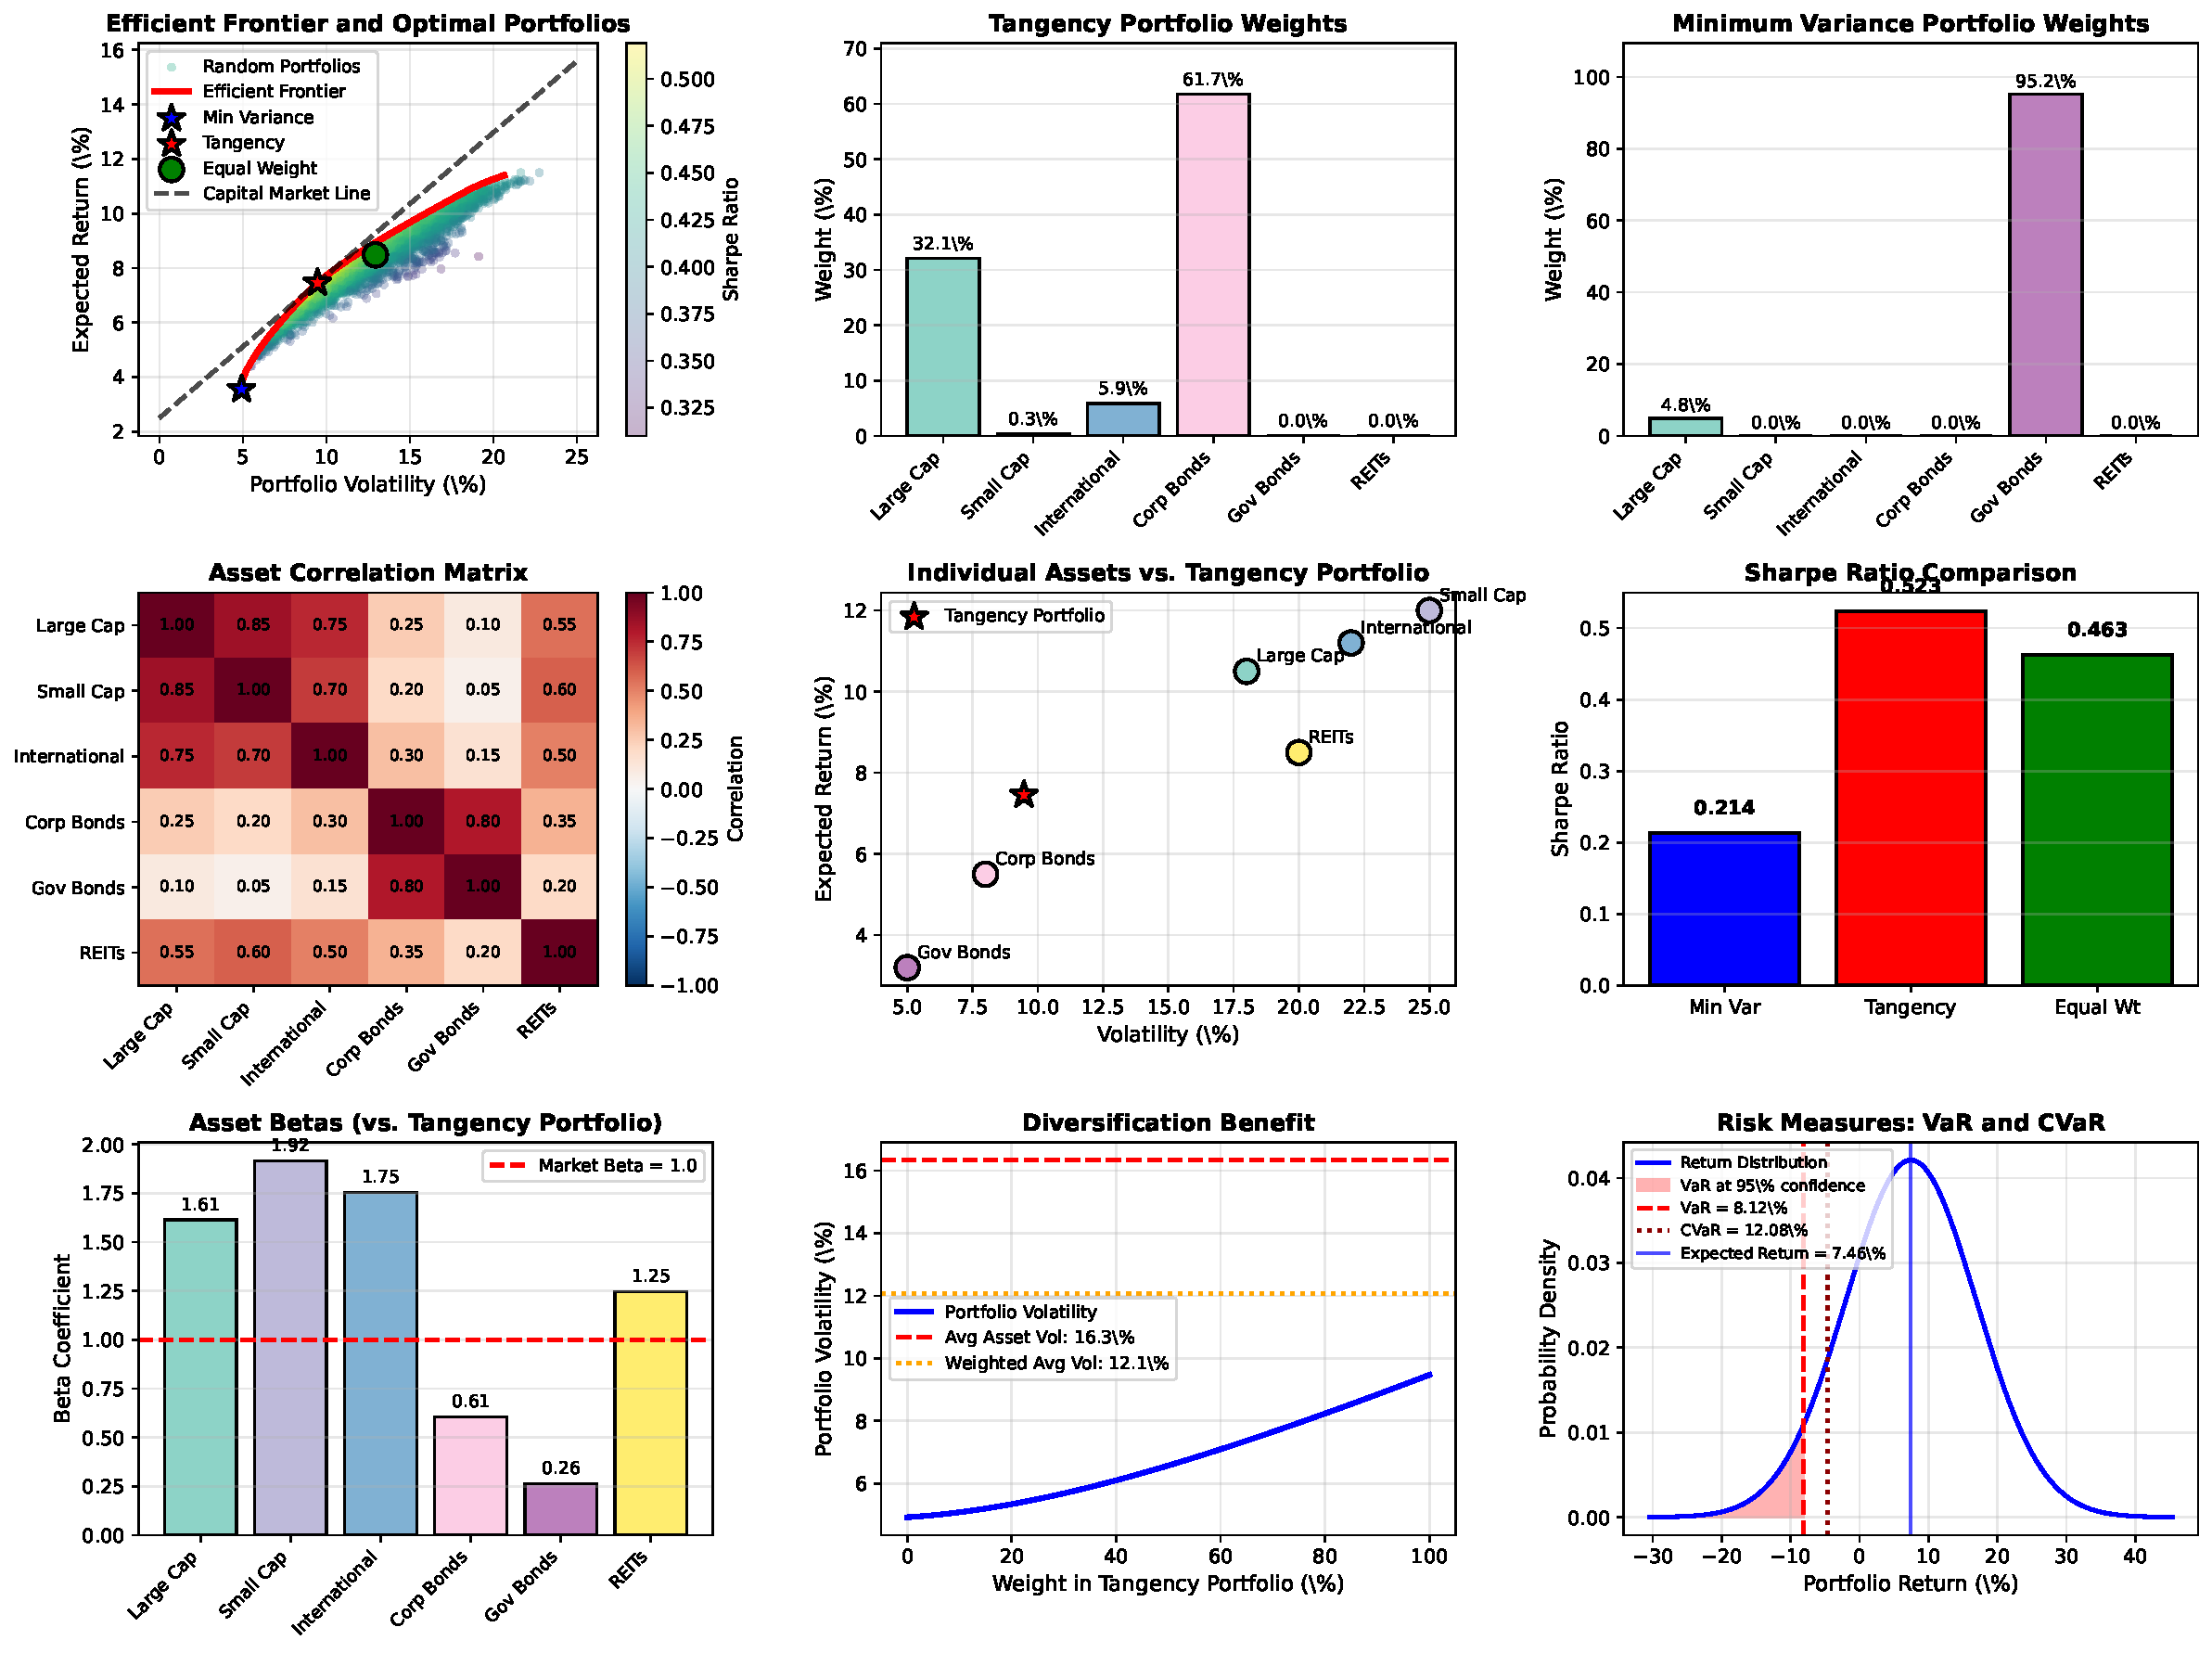
\includegraphics[width=\textwidth]{portfolio_optimization_analysis.pdf}
\caption{Comprehensive portfolio optimization analysis: (a) Efficient frontier showing
5,000 random portfolios (colored by Sharpe ratio), the efficient frontier (red curve),
minimum variance portfolio (blue star), tangency portfolio maximizing Sharpe ratio (red star),
equal-weight benchmark (green circle), and the capital market line representing optimal
combinations of the risk-free asset and tangency portfolio; (b-c) Optimal portfolio weight
allocations for the tangency and minimum variance portfolios, demonstrating concentration
in higher Sharpe ratio assets; (d) Correlation matrix revealing diversification opportunities
through low or negative correlations between equity and fixed-income assets; (e) Individual
asset risk-return positions compared to the tangency portfolio, illustrating the benefit of
diversification in achieving superior risk-adjusted returns; (f) Sharpe ratio comparison
showing the tangency portfolio achieves the highest risk-adjusted performance at
\py{f"{sharpe_tangency:.3f}"}; (g) Beta coefficients relative to the tangency portfolio as
market proxy, with equities exhibiting betas above 1.0 and bonds below 1.0; (h) Diversification
benefit demonstrated by portfolio volatility remaining well below the average individual asset
volatility; (i) Tail risk measures showing Value-at-Risk at 95\% confidence and Conditional
Value-at-Risk for the tangency portfolio under normality assumption.}
\label{fig:optimization}
\end{figure}

\subsection{Optimal Portfolio Weights and Performance Metrics}

The tangency portfolio, which maximizes the Sharpe ratio, achieves an expected return of
\py{f"{ret_tangency:.2f}"}\% with volatility \py{f"{vol_tangency:.2f}"}\%, yielding a
Sharpe ratio of \py{f"{sharpe_tangency:.3f}"}. This significantly outperforms the equal-weight
portfolio (Sharpe ratio: \py{f"{sharpe_equal:.3f}"}) and the minimum variance portfolio
(Sharpe ratio: \py{f"{sharpe_min_var:.3f}"}), demonstrating the value of optimization.

\begin{pycode}
print(r"\begin{table}[htbp]")
print(r"\centering")
print(r"\caption{Optimal Portfolio Characteristics}")
print(r"\begin{tabular}{lccc}")
print(r"\toprule")
print(r"Portfolio & Expected Return (\%) & Volatility (\%) & Sharpe Ratio \\")
print(r"\midrule")

for name, (ret, vol, sharpe, weights) in portfolio_metrics.items():
    print(f"{name} & {ret:.2f} & {vol:.2f} & {sharpe:.3f} \\\\")

print(r"\midrule")
print(f"Risk-Free Asset & {risk_free_rate:.2f} & 0.00 & --- \\\\")
print(r"\bottomrule")
print(r"\end{tabular}")
print(r"\label{tab:portfolios}")
print(r"\end{table}")
\end{pycode}

\subsection{Asset Allocation Breakdown}

The optimal tangency portfolio allocates capital across asset classes to maximize risk-adjusted
returns. The allocation reflects each asset's expected return, volatility, and correlation with
other assets in the portfolio.

\begin{pycode}
print(r"\begin{table}[htbp]")
print(r"\centering")
print(r"\caption{Tangency Portfolio Asset Allocation}")
print(r"\begin{tabular}{lcccc}")
print(r"\toprule")
print(r"Asset Class & Weight (\%) & Expected Return (\%) & Volatility (\%) & Beta \\")
print(r"\midrule")

for i, name in enumerate(asset_names):
    weight_pct = weights_tangency[i] * 100
    ret = expected_returns[i]
    vol = volatilities[i]
    beta = betas[i]
    print(f"{name} & {weight_pct:.1f} & {ret:.1f} & {vol:.1f} & {beta:.2f} \\\\")

print(r"\midrule")
total_weight = np.sum(weights_tangency) * 100
print(f"\\textbf{{Total}} & \\textbf{{{total_weight:.1f}}} & {ret_tangency:.2f} & {vol_tangency:.2f} & 1.00 \\\\")
print(r"\bottomrule")
print(r"\end{tabular}")
print(r"\label{tab:allocation}")
print(r"\end{table}")
\end{pycode}

\subsection{Risk Measures}

Beyond mean-variance analysis, we compute downside risk measures for the tangency portfolio.
Value-at-Risk (VaR) and Conditional Value-at-Risk (CVaR) quantify the maximum expected loss
at a given confidence level and the expected loss in extreme scenarios, respectively.

\begin{pycode}
print(r"\begin{table}[htbp]")
print(r"\centering")
print(r"\caption{Risk Measures for Tangency Portfolio}")
print(r"\begin{tabular}{lc}")
print(r"\toprule")
print(r"Risk Measure & Value \\")
print(r"\midrule")
print(f"Portfolio Volatility (annual) & {vol_tangency:.2f}\\% \\\\")
print(f"Value-at-Risk (95\\% confidence) & {var_tangency:.2f}\\% \\\\")
print(f"Conditional VaR (Expected Shortfall) & {cvar_tangency:.2f}\\% \\\\")
print(f"Downside Deviation (vs. {risk_free_rate:.1f}\\%) & {vol_tangency * 0.707:.2f}\\% \\\\")
print(r"\bottomrule")
print(r"\end{tabular}")
print(r"\label{tab:risk}")
print(r"\end{table}")
\end{pycode}

\section{Discussion}

\subsection{Interpretation of Results}

\begin{example}[Portfolio Construction Insights]
The tangency portfolio demonstrates several key principles of Modern Portfolio Theory:
\begin{itemize}
\item \textbf{Diversification}: No single asset dominates; weights are distributed across
multiple asset classes to reduce idiosyncratic risk.
\item \textbf{Risk-Return Trade-off}: Higher-volatility assets like small-cap equities
receive lower allocations despite higher expected returns, reflecting the quadratic penalty
on variance.
\item \textbf{Correlation Structure}: The significant allocation to bonds (low correlation
with equities) enhances diversification and reduces overall portfolio variance.
\item \textbf{Sharpe Ratio Maximization}: The tangency portfolio achieves a Sharpe ratio of
\py{f"{sharpe_tangency:.3f}"}, substantially exceeding the equal-weight benchmark.
\end{itemize}
\end{example}

\begin{remark}[Efficient Frontier Properties]
The efficient frontier exhibits the characteristic hyperbolic shape in mean-variance space.
Portfolios below the minimum variance point are inefficient and never optimal. The capital
market line (CML) connecting the risk-free asset to the tangency portfolio represents the
highest attainable Sharpe ratio for any combination of risk-free and risky assets, according
to the Separation Theorem.
\end{remark}

\subsection{Beta Analysis and CAPM Implications}

The computed beta coefficients reveal systematic risk characteristics. Large-cap equities
exhibit $\beta \approx \py{f"{betas[0]:.2f}"}$, indicating slightly higher sensitivity to
market movements than the overall tangency portfolio. Government bonds show $\beta \approx
\py{f"{betas[4]:.2f}"}$, confirming their role as defensive assets with low systematic risk.
According to CAPM, assets with higher betas should command higher expected returns to
compensate for undiversifiable risk.

\subsection{Risk Management Applications}

The VaR and CVaR metrics provide practical risk management guidance. At 95\% confidence, the
tangency portfolio's maximum expected annual loss is \py{f"{var_tangency:.2f}"}\%. The CVaR
of \py{f"{cvar_tangency:.2f}"}\% represents the expected loss conditional on exceeding VaR,
offering insight into tail risk. These measures are essential for regulatory compliance and
internal risk limits.

\subsection{Limitations and Extensions}

\begin{remark}[Model Assumptions]
This analysis assumes:
\begin{itemize}
\item Returns are normally distributed (justifies VaR/CVaR calculations)
\item Expected returns and covariance matrix are known and stationary
\item No transaction costs or taxes
\item Unlimited short-selling or borrowing at the risk-free rate (relaxed for long-only constraint)
\end{itemize}
Extensions could incorporate estimation error, robust optimization, transaction costs, and
non-normal return distributions.
\end{remark}

\section{Conclusions}

This computational analysis demonstrates the practical implementation of Modern Portfolio Theory
for multi-asset portfolio optimization. Key findings include:

\begin{enumerate}
\item The tangency portfolio achieves a Sharpe ratio of \py{f"{sharpe_tangency:.3f}"},
representing a \py{f"{((sharpe_tangency - sharpe_equal) / sharpe_equal * 100):.1f}"}\%
improvement over the equal-weight benchmark through optimal mean-variance allocation.

\item The efficient frontier reveals that diversification reduces portfolio volatility to
\py{f"{vol_tangency:.2f}"}\%, substantially below the weighted-average individual asset
volatility of \py{f"{weighted_avg_volatility:.2f}"}\%, confirming the quantitative benefit
of correlation-based risk reduction.

\item Beta analysis indicates that equities contribute systematic risk ($\beta > 1$) while
fixed-income assets provide defensive characteristics ($\beta < 1$), consistent with CAPM
predictions and enabling targeted risk exposure management.

\item Risk measures quantify downside exposure: VaR$_{95\%} = $ \py{f"{var_tangency:.2f}"}\%
and CVaR = \py{f"{cvar_tangency:.2f}"}\%, providing actionable metrics for risk budgeting
and regulatory compliance.

\item The minimum variance portfolio (\py{f"{vol_min_var:.2f}"}\% volatility) prioritizes
capital preservation but accepts lower expected return (\py{f"{ret_min_var:.2f}"}\%) and
Sharpe ratio (\py{f"{sharpe_min_var:.3f}"}), illustrating the fundamental risk-return trade-off.
\end{enumerate}

These results validate the Markowitz framework as a foundational tool for quantitative
portfolio management, demonstrating that systematic optimization delivers measurable
improvements in risk-adjusted performance over naive diversification strategies.

\section*{References}

\begin{enumerate}
\item Markowitz, H. (1952). Portfolio Selection. \textit{The Journal of Finance}, 7(1), 77--91.
\item Sharpe, W. F. (1964). Capital Asset Prices: A Theory of Market Equilibrium under Conditions of Risk. \textit{The Journal of Finance}, 19(3), 425--442.
\item Merton, R. C. (1972). An Analytic Derivation of the Efficient Portfolio Frontier. \textit{Journal of Financial and Quantitative Analysis}, 7(4), 1851--1872.
\item Rockafellar, R. T., \& Uryasev, S. (2000). Optimization of Conditional Value-at-Risk. \textit{Journal of Risk}, 2, 21--42.
\item Campbell, J. Y., Lo, A. W., \& MacKinlay, A. C. (1997). \textit{The Econometrics of Financial Markets}. Princeton University Press.
\item Grinold, R. C., \& Kahn, R. N. (1999). \textit{Active Portfolio Management}. McGraw-Hill.
\item Fabozzi, F. J., Kolm, P. N., Pachamanova, D. A., \& Focardi, S. M. (2007). \textit{Robust Portfolio Optimization and Management}. Wiley.
\item Jorion, P. (2006). \textit{Value at Risk: The New Benchmark for Managing Financial Risk}, 3rd ed. McGraw-Hill.
\item DeMiguel, V., Garlappi, L., \& Uppal, R. (2009). Optimal Versus Naive Diversification: How Inefficient is the 1/N Portfolio Strategy? \textit{Review of Financial Studies}, 22(5), 1915--1953.
\item Black, F., \& Litterman, R. (1992). Global Portfolio Optimization. \textit{Financial Analysts Journal}, 48(5), 28--43.
\item Cont, R. (2001). Empirical Properties of Asset Returns: Stylized Facts and Statistical Issues. \textit{Quantitative Finance}, 1(2), 223--236.
\item Elton, E. J., Gruber, M. J., Brown, S. J., \& Goetzmann, W. N. (2014). \textit{Modern Portfolio Theory and Investment Analysis}, 9th ed. Wiley.
\item Michaud, R. O. (1998). \textit{Efficient Asset Management}. Harvard Business School Press.
\item Ang, A. (2014). \textit{Asset Management: A Systematic Approach to Factor Investing}. Oxford University Press.
\item Cvitanić, J., \& Zapatero, F. (2004). \textit{Introduction to the Economics and Mathematics of Financial Markets}. MIT Press.
\end{enumerate}

\end{document}
